\documentclass[12pt,a4paper]{article}
\usepackage{microtype}
\usepackage{amsfonts}
\usepackage{amsthm}
\usepackage{graphicx}

\newcommand{\dpar}[1]{\left(#1\right)}

\newcommand{\N}{\mathbb{N}}
\newcommand{\R}{\mathbb{R}}

\theoremstyle{definition}
\newtheorem{ex}{Exercise}[section]

\title{Physics 1: Class 4}
\author{Max Jauregui}

\begin{document}
\maketitle

\section{Acceleration}

Let us consider a particle that moves along a straight line and let us
suppose that we know the velocities of the particle at the instants
$t_1$ and $t_2$. We define the \emph{average acceleration} of the
particle bewteen $t_1$ and $t_2$ as
$$\overline{a}=\frac{v(t_2)-v(t_1)}{t_2-t_1}\,.$$
In addition, we define the \emph{instantaneous acceleration} of the
particle at an instant $t$ by
$$a(t)=\lim_{\Delta t\to 0}\frac{v(t+\Delta t)-v(t)}{\Delta t}=\frac{dv}{dt}\,.$$
Since $v(t)=dx/dt$, it follows from the last equation that
$$a(t)=\frac{d}{dt}\dpar{\frac{dx}{dt}}=\frac{d^2x}{dt^2}\,,$$
where the last term is called the second derivative of the function
$x$ at the point $t$.

Since $a(t)$ is the derivative of the velocity at the instant $t$, in
a $v$ vs $t$ graph, $a(t)$ will be given by the slope of the line that
is tangent to the curve at the instant $t$. On the other hand, since
$a(t)$ is the second derivative of the position at the instant $t$, in
an $x$ vs $t$ graph, $a(t)$ will be given by the curvature of the
curve at the instant $t$. Basically, a curve has positive curvature at
a point if it has the form $\smile$ and negative curvature if it has
the form $\frown$. An inflection point of a curve is a point where the
curvature changes its sign. The curvature of the curve at this point
is zero.

\begin{ex}
  Let $x(t)=5t^3-10t+2$ be the position of a particle in meters, where
  $t$ is measured in seconds. Find the acceleration of the particle at
  the instant $1\,\mathrm{s}$. \emph{Answer:}
  $a(1)=30\,\mathrm{m/s^2}$.
\end{ex}

\begin{ex}
  Considering the $x$ vs $t$ graph given in Fig.~\ref{fig:xvst},
  answer the following:
  \begin{enumerate}
  \item[(i)] What are the signs of the acceleration between the
    instants $1\,\mathrm{s}$ and $2\,\mathrm{s}$?
  \item[(ii)] Is the acceleration negative in some instant between
    $4\,\mathrm{s}$ and $6\,\mathrm{s}$?
  \item[(iii)] What is the sign of the acceleration when the velocity
    of the particle attains its maximum value?
  \item[(iv)] Is there an instant where the acceleration is zero?
  \end{enumerate}
  \begin{figure}[ht]
    \centering
    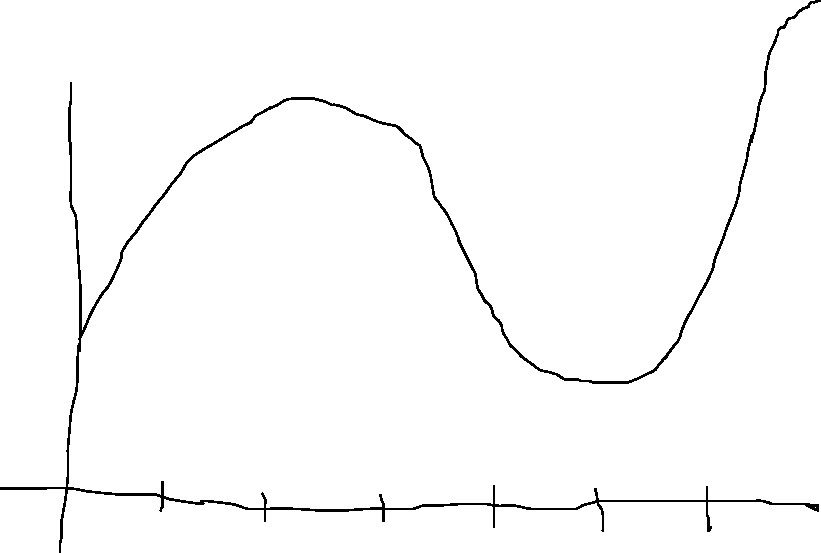
\includegraphics[width=0.5\textwidth,keepaspectratio]{figures/xvst.pdf}
    \caption{$x$ vs $t$ graph.}
    \label{fig:xvst}
  \end{figure}
\end{ex}

\section{Constant acceleration}

Let us consider a particle that moves in a straight line with constant
acceleration $a_0$, i.e., $a(t)=a_0$ for all $t\ge 0$. We will be
interested in obtaining the expression of the position of the particle
at an arbitrary instant $t$.

We begin by observing that, since $a(t)$ is the derivative of the
velocity at the instant $t$, in an analogous way to the case when we
obtained the position of a particle from the expression of its
velocity, we will have
$$v(t)-v(t_0)=\int_{t_0}^{t}a(t')\,dt'=a_0(t-t_0)\,.$$
Then,
\begin{equation}
  \label{eq:1}
  v(t)=v_0+a_0(t-t_0)\,,
\end{equation}
where $v_0=v(t_0)$.  Now, the displacement of the particle between two
instants $t_0$ and $t$ is given by
$$x(t)-x(t_0)=\int_{t_0}^{t}v(t')\,dt'=v_0(t-t_0)+\frac{a_0}{2}(t^2-t_0^2)-a_0t_0(t-t_0)\,.$$
Hence,
\begin{equation}
  \label{eq:2}
  x(t)=x_0+v_0(t-t_0)+\frac{a_0}{2}(t-t_0)^2\,,
\end{equation}
where $x_0=x(t_0)$.

From Eqs.~(\ref{eq:1}) and~(\ref{eq:2}) we can obtain other useful
equations. For instance, it follows from Eq.~(\ref{eq:1}) that
$$t-t_0=\frac{v(t)-v_0}{a_0}\,.$$
Using this in Eq.~(\ref{eq:2}), we can obtain that
$$v^2(t)-v_0^2=2a_0[x(t)-x_0]\,.$$
Moreover, using the expression of $a_0$, obtained from
Eq.~(\ref{eq:1}), we obtain
$$x(t)-x_0=\dpar{\frac{v(t)+v_0}{2}}(t-t_0)\,.$$

\end{document}
